\documentclass{standalone}
\usepackage[latin1]{inputenc}
\usepackage{tikz}
\usetikzlibrary{shapes, arrows}
% Define block styles
\tikzstyle{decision} = [diamond, draw, fill=blue!20, text width=6em,
    text badly centered, node distance=3cm, inner sep=0pt]
\tikzstyle{block} = [rectangle, draw, fill=blue!20, text width=5em, 
    text centered, rounded corners, minimum height=4em]
\tikzstyle{line} = [draw, -latex']
\tikzstyle{cloud} = [draw, ellipse,fill=red!20, node distance=3cm,
    minimum height=2em]
\tikzstyle{io} = [trapezium, trapezium left angle=70, trapezium right angle=110, 
    minimum height=1cm, text centered, draw=black, fill=blue!30]

\begin{document}
    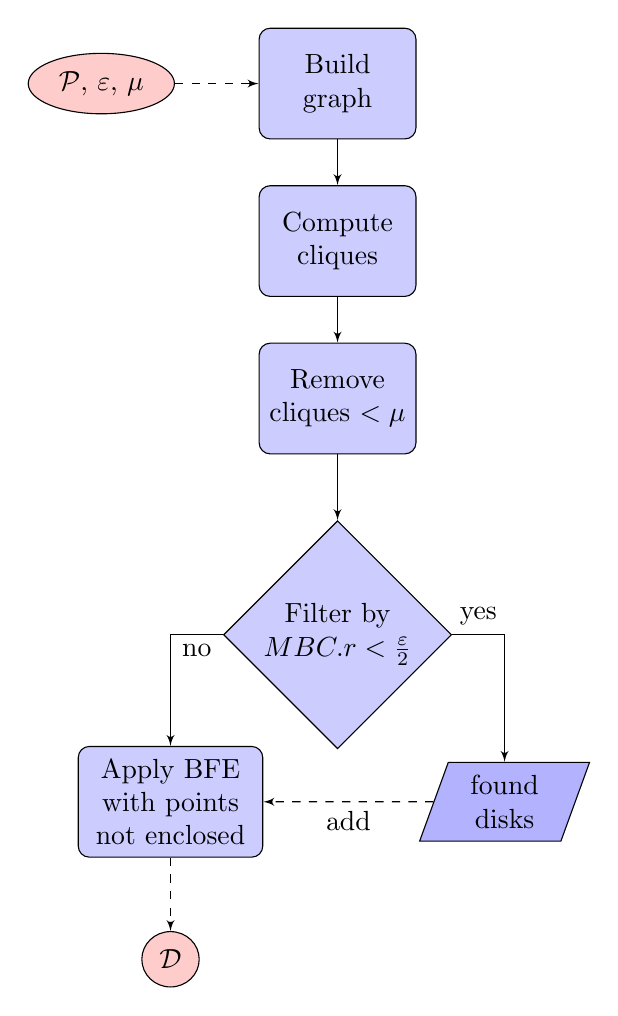
\begin{tikzpicture}[node distance = 2cm, auto]
        % Place nodes
        \node [block] (graph) {Build graph};
        \node [cloud, left of=graph, node distance=3cm] (input) {$\mathcal{P}$, $\varepsilon$, $\mu$};
        \node [block, below of=graph] (cliques) {Compute cliques};
        \node [block, below of=cliques, ] (filter) {Remove cliques $< \mu$};
        \node [decision, below of=filter] (decide) {Filter by $MBC.r < \frac{\varepsilon}{2}$};
        \node [io, below right of=decide, node distance=3cm, text width=3em] (disks1) {found disks};
        \node [block, below left of=decide, node distance=3cm, text width=6em] (traditional) {Apply BFE with points not enclosed};
        %\node [io, below of=traditional] (disks2) {disks2};
        %\node [io, below of=decide, node distance=4cm] (disks) {disks1 + disks2};
        %\node [block, below of=disks] (prune) {Prune disks};
        \node [cloud, below of=traditional, node distance=2cm] (maximals) {$\mathcal{D}$};
        % Draw edges
        \path [line,dashed] (input) -- (graph);
        \path [line] (graph) -- (cliques);
        \path [line] (cliques) -- (filter);
        \path [line] (filter) -- (decide);
        \path [line] (decide) -| node [near start] {yes} (disks1);
        \path [line] (decide) -| node [near start] {no}  (traditional);
        %\path [line] (traditional) -- (disks2);
        %\path [line] (disks1) |- (disks);
        %\path [line] (disks) -- (prune);
        \path [line,dashed] (disks1) -- (traditional) node[midway] {add};
        \path [line,dashed] (traditional) -- (maximals);
    \end{tikzpicture}
\end{document}
